\documentclass[/home/greg/Thesis/main/main.tex]{subfiles}

% Default image directory
\def\thisdir{/home/greg/Neutron_star_modelling/TimingNoiseModels/InTheRotatingFrame}
\graphicspath{{/home/greg/Neutron_star_modelling/TimingNoiseModels/InTheRotatingFrame/img/}}

\begin{document}

\section{Defining the model}

The rotation of a rigid body in the rotating reference frame is described by
Euler's equations. To derive these, we begin with Euler's second law  for the
angular momentum $\mathbf{L}$ in the interial frame

\begin{equation}
    \frac{d\mathbf{L}}{dt}=\mathbf{T},
\end{equation}

where $\mathbf{T}$ is the applied torque. The angular momentum can be written
as $I \spin$, the product of the moment of interia tensor and the spin vector.
In the inertial frame both of these quantities vary in time; this does not lend
itself to solving the equations. We can simplify solutions by transforming to a
frame fixed in the rotating frame of the rigid body and aligning the axes with
the principle axes of $I$. In such as frame the moment of inertia is constant
and diagonal. The transformation to a rotating reference frame requires a
modification of the time derivative in Euler's second law, see \citet{Landau1969}
for details. The result is Euler's rigid body equations in the rotating frame:
\begin{equation}
    \frac{d\mathbf{L}}{dt} + \spin \times \mathbf{L} = \mathbf{T}.
    \label{eqn: eom}
\end{equation}
To begin with, we will restrict ourselves to consider only biaxial bodies with 
principle moments given by
\begin{equation}
I_{x} = I_{y} = I_{0} \;\;\;\;\;\;\; I_{z} = I_{0}(1+\epsilon_{I}),
\end{equation}
where $I_{0}$ is the moment of inertia for which we use a canonical value of 
\begin{equation}
I_{0} = \frac{2}{5}MR^{2} \approx 10^{45}\textrm{g cm}^{2} M_{1.4}R_{6}^{2}.\footnote{$M_{1.4}$ is mass in units of $1.4 M_{\odot}$ and $R_{6}$ is the radius in units of $10^{6}$cm}
\end{equation}
Equation \ref{eqn: eom} gives us three coupled ODEs for $\omega_{x}, 
\omega_{y}$ and $\omega_{z}$. In the torque-free case analytic solutions can be
found. If the spin-vector is initially at some angle to the $\z$ axes, it will
rotate in a cone about the $\z$ axes. This motion in referred to as free precession
and the period is given by 
\begin{equation}
    \tau_{p} = \frac{1}{\epsilon_{I}\nu_{0}},
    \label{eqn: fp timescale}
\end{equation}
where $\nu_{0} = \omega_{0}/2\pi$ is the initial spin frequency. 

We now will not include a torque modelling a dipole $m$ frozen into the star in
the $\x-\z$ plane at an angle $\chi$ to the $\z$ axis. \citet{Deutsch1955}
demonstrated such a dipole exerts a torque on the star which has two
components. It is presented here in form found in \citet[hereafter
G70]{Goldreich1970}.
\begin{equation}
\boldsymbol{T}=\frac{2R}{3c} I_{0}\epsilon_{A}\omega^{2}
               (\spin \times \hat{\boldsymbol{m}})\times \hat{\boldsymbol{m}} 
               + \epsilon_{A}I_{0}(\spin \cdot \hat{\boldsymbol{m}})
               (\spin \times \hat{\boldsymbol{m}}), \;\;\;\;\; \textrm{ with } 
               \;\;\;\; \epsilon_{A} = \frac{m^{2}}{I_{0}R_{6}c^{2}},
\label{eqn: torque}
\end{equation}
where $\epsilon_{A}$ the magnetic deformation as defined by \citet{Glampedakis2010}.
The first term on the right hand side is often referred to as the \emph{spin
down}, or \emph{braking} torque. As this suggests it is responsible for the
power law retardation of spin frequency and has an associated timescale
$\tau_{S}$. The second term is known as the \emph{anomalous} torque which acts
on a timescale $\tau_{A}$. These time scales are given by 
\begin{equation}
\tau_{A}=\frac{1}{\epsilon_{A}\nu_{0}},  \;\;\;\;\; 
\tau_{S}=\frac{3c}{2R}\frac{1}{\epsilon_{A}\nu_{0}^{2}},
\label{eqn: torque timescales}
\end{equation}• 

We now have the basic components of out neutron star: a biaxial rigid body 
spundown by a dipole torque. In table~\ref{tab: definitions} we list the
relevant angles of each component and a sketch is provides in
figure~\ref{fig: sketch01}. 

\begin{table}[ht]
\centering
\begin{tabular}{|l|c|c|c|c|} \hline
 \multicolumn{2}{|c|}{} & Magnitude & Polar angle & Azimuthal angle \\ \hline
Spin vector  & $\boldsymbol{\omega}$ & $\omega$ & $a$ & $\phi$ \\ \hline
Magnetic dipole &  $\boldsymbol{m}$ & $m$ & $\chi$ & 0 \\ \hline
\end{tabular}•
\caption{Table of spherical components for the spin vector and magnetic dipole}
\label{tab: definitions}
\end{table}

\begin{figure}[ht]
\centering
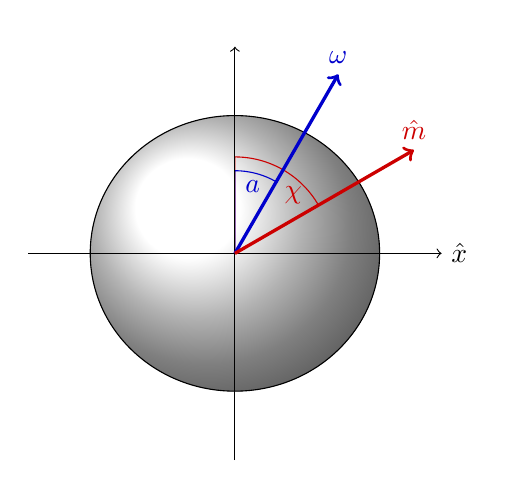
\begin{tikzpicture}[scale=1.75] 
	% Define some things

	\def\costhirty{0.8660256}
	\def \mag{1.5}

	\def\cosbeta{0.984}
	\def\sinbeta{0.173}

	% Colors
	\colorlet{anglecolor}{blue!80!black}
	\colorlet{sincolor}{red}
	\colorlet{tancolor}{orange!80!black}
	\colorlet{coscolor}{blue}

	% Styles
	\tikzstyle{axes}=[]
	\tikzstyle{important line}=[very thick]
	\tikzstyle{information text}=[rounded corners,fill=red!10,inner sep=1ex]

	% Draw the shaded star
	\def\R{1.0} % sphere radius
	\filldraw[ball color=white] (0,0) ellipse (1.05 and 1.0);

	% Draw the angles
	\draw[draw=red!80!black] (0,0) -- (0pt,7mm) arc(90:30:7mm);
	  \draw (45:6mm) node[red!80!black] {$\chi$};


	\draw[draw=blue!80!black] (0,0) -- (0pt,6mm) arc(90:60:6mm);
	  \draw (75:5mm) node[blue!80!black] {$a$};



	%\draw[draw=green!60!black] (0,0) -- (12mm*\costhirty,12mm*0.5) arc(30:60:12mm);
	 % \draw (45:11mm) node[green!60!black] {$\alpha$};



	% Draw the body frame axis
	\draw[->] (-1.5,0) -- (1.5,0) node[right] {$\hat{x}$};
	\draw[->] (0,-1.5) -- (0,1.5) node[above] {$\z$};

%	% Draw the effective body frame axis
%	\draw[draw=black] (0,0) -- (0,13mm) arc(90:100:13mm);
%%	  \draw (95:11mm) node[black] {$\beta$};
%	\draw[draw=magenta] (0,0) -- (-8.1*\sinbeta mm, 8.1*\cosbeta mm) arc(100:60:8.1mm);
%	  \draw (80:9.2mm) node[magenta] {$a'$};
%
%	\draw[dashed,->] (-1.5*\cosbeta,-1.5*\sinbeta) -- (1.5*\cosbeta,1.5*\sinbeta) node[right] {$x'$};
%	\draw[dashed,->] (1.5*\sinbeta,-1.5*\cosbeta) -- (-1.5*\sinbeta,1.5*\cosbeta) node[above] {$z'$};




	% Define omega to have unit magnitude and lie at 30 degrees to the z axis
	{\draw[color=blue!80!black,very thick,->] (0,0,0) -- (\mag*0.5,\mag*\costhirty) node[anchor=south]{$\omega$};}%

	% Define m to have unit magnitude and lie at 60 degrees to the z axis
	{\draw[color=red!80!black,very thick,->] (0,0,0) --(\mag*\costhirty,\mag*0.5) node[anchor=south]{$\hat{m}$};}%

\end{tikzpicture}

\caption{Sketch of the  $\x-\z$ plane,  the magnetic dipole lies solely in
    this plane, it's azimuthal component is always zero.  Only the projection
into this plane of the spin vector is shown, in general it has an azimuthal
component given by $\phi$.}
	\label{fig: sketch01}
\end{figure}•

We will now present results of this model found using numerical intergration
of \eqref{eqn: eom} with the torque defined in \eqref{eqn: torque}. 

\FloatBarrier
\section{Spherical star}
\label{sec: spherical}

As a first validation that the model agrees with analytic calculations we solve
for a spherical star $\epsilon_{I}=0$. In such a case the star will not precess.
This model was first considered by \citet{Davis1970}
and separately by \citet{Michel1970}; both sets of authors discovered that the
spin axis aligns with the magnetic axis on the spindown timescale. This is
incompatible with the observation of neutron stars as NSs as we need the
dipole to be misaligned with the spin axes to observe pulses. 

We set $\chi=30^{\circ}$ and $\epsilon_{A}=5\times10^{-11}$ and plot the
components of the spherical components spin vector in figure~\ref{fig: NS
spherical}. This shows a brief spin down which halts once the spin vector
aligns with the magnetic dipole $a \rightarrow \chi=30^{\circ}$.  The azimuthal
angle $\phi$ does not vary, this is expected since precession, a monotonic
increase in $\phi$, does not occur for spherical bodies. This result agrees
with the analytic calculations: the allignment occurs on the spin down time
scale $\sim 3.6\times 10^{8}$.
\begin{figure}[ht]
\centering
	\centering
	\includegraphics[width=0.5\textwidth]
     {{Spherical_Plot_no_anom_chi_30.0_epsI_0.0_epsA_5.0e-11_omega0_1.0e4_t1_1e8}.png}
\caption{Plot of the spherical components of $\boldsymbol{\omega}$ for a
spherical star. Note that the magnetic dipole is inclined at $\chi=30^{\circ}$
to the $\z$ axis.}
\label{fig: NS spherical}
\end{figure}•

\FloatBarrier
\section{Biaxial NS with no anomalous torque}
We begin with the evolution of the spin vector neglecting the anomalous torque.
This reduces the number of timescales to just two, the spin down and the
precession timescale. The solutions are categorised by the ordering of these
time scales; it is shown  in appendix \ref{sec: timescales} that these orderings
remain valid for the duration of the spindown. The ordering of the two timescales
gives three different types of solutions corresponding to three regions:
\begin{align}
    \textrm{Regions A: } \tau_{S} > \tau_{P} &&& 
    \textrm{Region B: } \tau_{S} \sim \tau_{P} &&& 
    \textrm{Resgion C: } \tau_{S} < \tau_{P}
\end{align}
Since all solutions in each region display the same behaviour, we pick three 
`neutron stars (NS)' and list their parameters in table \ref{tab: A B C params}. 

\renewcommand{\arraystretch}{1.2}
\begin{table}[htb]
\centering
{\small
	\begin{tabular}[h]{|l|c|c|c|c|c|}\hline
		&  $\epsilon_{I}$  & $\epsilon_{A} $ & 	$B_{S} \; $[Gauss] & $\tau_{S}$ [s] & $ \tau_{P}$  [s] \\ \hline
	NS A 	&  $  1.0\times 10^{-9}  $  & $  0.5\times 10^{-10}  $ & 	$  1.3\times 10^{13}  $   & $  3.6\times 10^{8}  $ & $  6.3\times 10^{5}  $\\
	NS B 	&  $  0.4\times 10^{-10}  $  & $  0.5\times 10^{-10}  $ & 	$  1.3\times 10^{13}  $   & $  3.6\times 10^{8}  $ & $  1.6\times 10^{7}  $\\ 
	NS C 	&  $  1.0\times 10^{-15}  $  & $  0.5\times 10^{-10}  $ & 	$  1.3\times 10^{13}  $   & $  3.6\times 10^{8}  $ & $  6.3\times 10^{11}  $\\ \hline
	\end{tabular}
}
\caption{Table of relevant values for the selected points. In calculating the
    Magnetic fields we have assumed canonical value of $R=1\times10^{6}$cm for
    the radius, and a value $\omega_{0} = 1\times10^{4}$ rads $s^{-1}$}
\label{tab: A B C params}
\end{table}

\subsubsection{Phase space}
The phase space of solutions is plotted in figure~\ref{fig: phase space no anom}
parametrised by the elastic deformation $\epsilon_{I}$ and the surface magnetic
field $B_{S}$ which is given by~\citep[][ p. 278]{Shapiro83}
\begin{equation}
B_{S} = \frac{2m}{R^{3}}
\end{equation}•

\begin{figure}[ht]
\centering
\includegraphics[scale=0.5]{{phase_space_no_anom}.png}
\caption{Phase space of solutions categorised by the ordering of the two
    timescales as a function of the elastic deformation $\epsilon_{I}$ and the
    surface magnetic fields $B_{s}$.}
\label{fig: phase space no anom}
\end{figure}

Without the anomalous torque the ordering of the timescales defines  two
distinct regions separated by $\tau_{S}=\tau_{P}$. To aid the speed of
numerical calculation  an unrealistic value of the initial spin frequency
$\omega_{0}=10^{4}$[rads $s^{-1}$] is used. Using a more realistic value the
type of solution remains the same only the time scales vary. A comparison of
this phase space with the true NS population in section~\ref{sec: Connection
with the known NS population}.

The elastic deformation $\epsilon_{I}$ may take either a positive or a negative
values; these correspond to either an oblate or prolate mass distribution.
 In all of the following we use only positive values of
$\epsilon_{I}$ as these are thought to be more physical. It will be noted when
this is thought to be important. Finally we must choose the angle between the
magnetic dipole and the elastic deformations $\chi$, because of the symmetry of
the star about the $\z$ axis we choose two values $30^\circ$ and $75^\circ$ to
demonstrate important cases. Initial conditions are thought to have some
bearing on the solutions \citep[see][]{Melatos2000}. In the current work we
will start with the spin vector having inclination angle of $50^{\circ}$ and
azimuth $0^{\circ}$.


\FloatBarrier


\FloatBarrier \subsection{NS A in region $\tau_{S}\gg \tau_{P}$}
\label{sec: A_NA} 
NSs in this region are described by the work of
\citetalias{Goldreich1970}. In addressing the shortcomings of the analytic spherical solutions,
Goldreich considered a neutron star with a solid crust capable of supporting
elastic strains. In order to find an analytic solution Goldreich assumed that
the precession timescale was significantly shorter than the spin down
timescale. Averaging equations \eqref{eqn: eom} with this assumptions yields
\begin{eqnarray}
\Big\langle \frac{d \omega}{dt}\Big\rangle & = & -\frac{2R}{3c}\epsilon_{a}\omega^{3}\left[ \sin^{2} \chi +\sin^{2}a \left(1-\frac{3}{2}\sin^{2}\chi\right)\right], \\
\Big\langle \frac{d a}{dt}\Big\rangle & = & -\frac{2R}{3c}\epsilon_{a}\omega^{2}\sin a \cos a \left(1-\frac{3}{2}\sin^{2}\chi\right).
\label{eqn: goldreich_averaged_eqns}
\end{eqnarray}•
These expression indicate that the polar angle $a$ will either grow or decay on
the spindown timescale depending on whether $\chi$ was greater or less than
$\approx 55^{\circ}$. 

We first present results for all the spherical components during the spindown 
in figure~\ref{fig: NS A_NA}. For the angle $\chi$ we use two values
$30^{\circ}$ and $75^{\circ}$ and find that $a$ tends to either $0$ or $\pi/2$
on the spindown timescale as suggested by \citetalias{Goldreich1970}.
During this alignment, the spin magnitude decays
and $\phi$ monotonically increases corresponding to the spin vector precessing
about the $\z$ axis. 
\begin{figure}[ht]
\centering
\begin{tabular}{cc}
	\subfloat[$\chi=30^{\circ}<\chi_{cr}$]{\includegraphics[width=0.495\textwidth]
             {{Spherical_Plot_no_anom_chi_30.0_epsI_1.0e-9_epsA_5.0e-11_omega0_1.0e4_eta_1.0e-4}.png}} & 
    \subfloat[$\chi=75^{\circ}>\chi_{cr}$]{\includegraphics[width=0.495\textwidth]
             {{Spherical_Plot_no_anom_chi_75.0_epsI_1.0e-9_epsA_5.0e-11_omega0_1.0e4_eta_1.0e-4}.png}}
\end{tabular}•
\caption{Plot of the spherical components of $\boldsymbol{\omega}$ for NS
A. The two choices of $\chi$ allow us to confirm Goldreich's dependence of the
alignment of the spin vector on $\chi$.  }
\label{fig: NS A_NA}
\end{figure}•

We investigate the differences beween Goldreich's averaged equations
\eqref{eqn: goldreich_averaged_eqns} and the exact solution without averaging
in figure~\ref{fig: NS A_NA comparison}.

\begin{figure}[ht]
\centering
\begin{tabular}{cc}
    \subfloat[$\chi=30^{\circ}<\chi_{cr}$]{\includegraphics[width=0.495\textwidth]
             {{Plot_a_averaged_and_exact_chi_30}.png}} & 
    \subfloat[$\chi=75^{\circ}>\chi_{cr}$]{\includegraphics[width=0.495\textwidth]
             {{Plot_a_averaged_and_exact_chi_75}.png}}
\end{tabular}
\caption{Plot of the angle $a$ for both the exact solution of \eqref{eqn: eom}
and the solution to the averaged equations \eqref{eqn: goldreich_averaged_eqns}.}
\label{fig: NS A_NA comparison}
\end{figure}•
Our model agrees well with Goldreich's averaged result, but
also exhibits oscillations due to precession. 
\FloatBarrier

\paragraph{A geometric argument}
To better understand the evolution of the spin vector and in particular the
significance of $a \sim 55^{\circ}$ we introduce a geometric argument. 
Writing the conservations of energy and momentum in terms
of the angular momentum vector $J_{i}$ for a biaxial mass distribution we have 
\begin{eqnarray}
1 & = & \frac{J_{x}^{2}}{2I_{x}E}+\frac{J_{y}^{2}}{2I_{y}E}+\frac{J_{z}^{2}}{2I_{z}E} =  \frac{J_{x}^{2}}{2I_{0}E}+\frac{J_{y}^{2}}{2I_{0}E}+\frac{J_{z}^{2}}{2I_{0}(1+\epsilon_{I})E},\\
J^{2} & = & J_{x}^{2}+J_{y}^{2}+J_{z}^{2}.
\label{eqn: sphere ellipsoid biaxial}
\end{eqnarray}•
The first equation describes a biaxial ellipsoid with semi-axis given by
$\sqrt{2I_{0}E}$, $\sqrt{2I_{0}E}$ and $\sqrt{2I_{0}(1+\epsilon_{I})E}$.  The
second describes a sphere of radius $J$. Both shapes are concentric with their origin
at $\boldsymbol{0}$. Physical solutions require the conservation of both the energy
and momentum, these solutions are therefore the intersection of the sphere and 
ellipsoid. This bounds the radius of the sphere by
\begin{equation}
2EI_{0}<J^{2}<2EI_{0}(1+\epsilon_{I}).
\end{equation}•
For a fixed energy and momentum, the intersection describes a circle about the
$\z$ axis. Several typical intersections are shown in figure~\ref{fig: plot
sphere ellipse biaxial}. Points on the circle are the set of all possible
solutions to the conservation equations for the angular momentum vector
$J_{i}$. Since $J_{i}=I_{ij}\omega^{j}$ and the moment of inertia tensor is
static, numerical solutions for the spin vector must also exist as points on a
related circle. This related circle is exactly the precession of $\spin$ about
the $\z$ axis.

Both the energy and the momentum decay exponentially in time
due to the spindown. As a result both the sphere and ellipsoid will shrink, but
not necessarily at the same rate. If we imagine observing the ellipsoid such
that it appears to be fixed, we may see the sphere either shrink or grow with
respect to the ellipsoid. We can parameterise the relative rate of shrinking by
considering the quantity
\begin{equation}
A(t)  = \frac{J^{2}} {2EI_{0}} 
\label{eqn: A}
\end{equation}•
We could have chosen any one of the ellipsoids semi-axis since they are all
proportional up to constants of $\epsilon_{I}$. The evolution of the spin
vector is related to the rate of change of $A$.
This quantity determines whether the sphere shrinks or grows with respect to
the ellipsoid. It is worth taking a moment to understand the different cases
which are parametrised by the sign of $\dot{A}$:
\begin{enumerate} 
\item $\dot{A}>0$ The sphere grows with respect to the ellipsoid. In this case
    the intersection circles will `close up' around the $\z$ axis. This
    agrees with the solution for $\chi=30^{\circ}$ given in
    figure~\ref{fig: NS A_NA comparison}(a). The angle between
    $\boldsymbol{\omega}$ and the $\z$ axis tends to zero while $\phi$
    monotonically increases. This describes the spinvectors following a circle 
    about the $z$ axis which gradiuall decreases in radius.
\item $\dot{A}<0$ The sphere shrinks with respect to the ellipsoid. In this
    case the intersection circles will increase in radius until $J\rightarrow
    \sqrt{2EI_{0}}$. This describes exactly the solution in
    figure~\ref{fig: NS A_NA comparison}(b): that is $a\rightarrow
    90^{\circ}$ while $\phi$ monotonically increases.
\end{enumerate}•

\begin{figure}[ht]
\centering
\includegraphics[trim = 50mm 50mm 50mm 20mm, clip=true ,scale=0.8]{{Ellipsoid_Sphere_Biaxial}.pdf}
\caption{Intersection of the sphere and ellipsoid defined in equations
    \eqref{eqn: sphere ellipsoid biaxial} for three different values of $M$ at
fixed $E$. The sphere's of radius $M$ are not visible, only the blue line shows
where they would intersect the fixed ellipsoid.}
\label{fig: plot sphere ellipse biaxial}
\end{figure}•
\FloatBarrier

\paragraph{Connecting with Goldreich's result}
In appendix \ref{sec: goldreich} we verify that the time averaged rate of change
of $A$ is given by the following.
\begin{equation}
\langle \dot{A} \rangle =\frac{1}{\langle E\rangle ^{2}}I_{0}^{2}\epsilon_{I}
                          \omega^{6}\frac{2R}{3c}\epsilon{A} \cos^{2} a 
                          \sin^{2}a\left(1-\frac{3}{2}\sin^{2}\chi\right) 
\end{equation}
This result is valid only in the regime for which $\tau_{S}\gg \tau_{P}$ and
neglects the anomalous torque and term of order $\epsilon_{I}^{2}$. It
demonstrates that only two factors determine the sign of $\dot{A}$: the sign of
$\epsilon_{I}$ and the term $1-\frac{3}{2}\sin^{2}\chi$ giving a critical value
$\chi_{cr}\approx55^\circ$. The first we should expect on geometric grounds, a
change in sign of the deformation changes the geometry of the ellipsoid. The
second is in perfect agreement with the findings of G70, and shows that this
critical value is a tipping point between the rates of change of energy and
angular momentum.

%\paragraph{Connecting with the numeric results}
%We can now interpret our numerical solutions as the evolution of these circles,
%the spin vector is constrained to lie on the circle as it evolves. To
%understand if the sphere shrinks or grows with respect to the ellipsoid we plot
%the quantity $A$ for both values of chi in figure~\ref{fig: NS A A} using
%$\epsilon_{I}=0.1$ for illustrative purposes. It is clear from this that the
%sphere grows with respect to the ellipsoid for $\chi=30^{\circ}$, and shrinks,
%reaching unity at late times for $\chi=75^{\circ}$.
%
%
%
%\begin{figure}[ht]
%\centering
%\includegraphics[scale=0.4]{{NS_A_NA_Combined_A}.png}
%\caption{Plot of the quantity $A$ defined in equation \eqref{eqn: A} for NS A without the anomalous torque. So that the effect is visible a value of $\epsilon_{I}=0.1$ has been used rather than $\epsilon_{I}=1\times10^{-9}$ in the post-processing only. } 
%\label{fig: NS A A}
%\end{figure}•


\paragraph{Summary} We find that, without the anomalous torque, the numerical
model agrees well with analytic results in the literature. Further, we give an
intepretion of the critical value of $chi$ found by \citetalias{Goldreich1970}.

\FloatBarrier
\subsection{NS B in region $\tau_{S}\sim \tau_{P}$}
\label{sec: B_NA}
Unlike the previous examples, there is no comparison in the literature which
considers $\tau_{P}\sim\tau_{S}$ while neglecting the anomalous torque. This is
primarily because the similarity of the timescales means simplifying
assumptions cannot be made. The results have not been included here as they are
exactly alike with the results of NS A, except the similarity of time
scales means both the precession and alignment of the spin vector occur on the
same timescale.

\FloatBarrier
\subsection{NS C in region $\tau_{S}\ll \tau_{P}$}
\label{sec: C_NA}
In NS C the timescales take the ordering $\tau_{P}\gg \tau_{S}$. An analogy
can be made that the limit of this region, is the spherical star
($\epsilon_{I}\rightarrow0$) discussed in section~\ref{sec: spherical}. Solving
the equations of motion for NS C the spherical components of the spin axis
are given in figure~\ref{fig: NS C_NA}. Both choices of $\chi$ yield a
similar result, the polar angle $a$ tends to $\chi$ on the spin down timescale
as anticipated by the likeness to the spherical star. In contrast the azimuthal
angle $\phi$ appears to begin monotonically increasing before approaching a
constant, it is thought that this is due to the small but not vanishing
magnitude of $\epsilon_{I}$. In the perfectly spherical limit we observe no
such increase in $\phi$. Therefore the small
deformation offsets the steady state solution of the spin axis from the
magnetic dipole. 

For an intuitive understanding consider that the torque acts to align the spin
axis with the magnetic dipole; when this occurs the torque vanishes. Since the
mass is not spherical, stable solutions exist only when the spin vector aligns
with the principle axis of the moment of inertia tensor $\x,\y$ and $\z$. So
when both effects act, the steady state solution is an intermediary point
between the two weighted by the relative strength of each effect. In this case
the torque dominates and so the spin vector lies close, but not exactly
aligned, with the magnetic dipole. During this time the star spins down but
upon alignment the spin frequency asymptotically approaches a constant non zero
value. 
%We also plot in figure~\ref{fig: NS C_NA alpha} the angle between the spin axis and magnetic dipole $\alpha$ for NS C confirming the previous findings. 
\begin{figure}[ht]
\centering
\begin{tabular}{cc}
    \subfloat[$\chi=30^{\circ}<\chi_{cr}$]{\includegraphics[width=0.495\textwidth]{{Spherical_Plot_no_anom_chi_30.0_epsI_1.0e-15_epsA_5.0e-11_omega0_1.0e4_t1_1e8}.png}}&
    \subfloat[$\chi=75^{\circ}>\chi_{cr}$]{\includegraphics[width=0.495\textwidth]{{Spherical_Plot_no_anom_chi_75.0_epsI_1.0e-15_epsA_5.0e-11_omega0_1.0e4_t1_1e8}.png}}
\end{tabular}
\caption{Plot of the spherical components of $\boldsymbol{\omega}$ for NS C. }
\label{fig: NS C_NA}
\end{figure}•

\FloatBarrier

\section{Biaxial NS including the anomalous torque}
We now include the anomalous torque component in equation \eqref{eqn: eom} and
discuss the differences this makes to the numerical solutions. Before doing
this we consider the appropriate reference frame in which to view the system.

\subsection{Effective body frame} 
Working with a biaxial body and the Deutsch torque 
\cite{Melatos2000} discovered non-trivial solutions where the spin axis aligns with
an unkown angle between the magnetic dipole and the principle axis of the MOI.
This was interpreted by Melatos as evidence for persistent precession. We show 
in section \ref{sec: B} that in fact the spin vector is aligning with another
rotating reference frame that is held at a fixed angle to the original rotating
reference frame. This reference frame, which we label the \emph{effective} body
frame is a result of the inclusion of the anomalous torque.

Writing equation~\eqref{eqn: eom} with the Deutsch torque we have:
\begin{eqnarray*}
J^{i}_{\;,t}+\epsilon^{ijk}\omega_{j}J_{k} & = 
& N^{i}_{\textrm{spin down}}+
\epsilon_{A}I_{0}\omega^{a}\hat{m}_{a}\epsilon^{ijk}\omega_{j}\hat{m}_{k}, \\
J^{i}_{\;,t}+
\epsilon^{ijk}\omega_{j}\left(J_{k}-\epsilon_{A}I_{0}\omega^{a}\hat{m}_{a}\hat{m}_{k}\right) 
& = & N^{i}_{\textrm{spin down}}, \\
J^{i}_{\;,t}+
\epsilon^{ijk}\omega_{j}\left(I_{ka}-\epsilon_{A}I_{0}\hat{m}_{a}\hat{m}_{k}\right)\omega^{a} 
& = & N^{i}_{\textrm{spin down}}. 
\end{eqnarray*}•
By separating the equation this way and making use of $J_{i}=I_{ij}\omega^{j}$
we can write an effective moment of inertia tensor given by 
\begin{eqnarray}
I'_{jk}&=&I_{jk}-I_{0}\epsilon_{A}\hat{m}_{j}\hat{m}_{k}, \\
&=& \left[ 
\begin{array}{ccc}
I_{0}(1-\epsilon_{A}\sin^{2}\chi) & 0 & -I_{0}\epsilon_{A}\sin\chi \cos \chi \\  
0 & I_{0} & 0 \\  -I_{0}\epsilon_{A}\sin\chi \cos \chi& 0 &  
I_{0}(1+\epsilon_{I}-\epsilon_{A}\cos^{2}\chi)
\end{array}
\right].
\label{eqn: effective MOI}
\end{eqnarray}•
Note we will use the prime to denote the effective body frame axis when quoting
results. This effective moment of inertia tensor can be shown to have
eigenvalues given by 
\begin{equation}
\lambda_{2}=I_{0}, \;\;\; \lambda_{\pm}=\frac{I_{0}}{2}\left(2+\epsilon_{I}-\epsilon_{A}\pm \sqrt{\epsilon_{A}^{2}+\epsilon_{I}^{2}-2\epsilon_{A}\epsilon_{I}\cos(2\chi)}\right).
\end{equation}•
If we diagonalise this effective moment of inertia tensor, these eigenvalues
are the diagonal entries, and the associated eigenvectors are the principle
axis of the effective body frame axis. The eigenvalues always take the ordering
\begin{equation}
\lambda_{+}>I_{0}>\lambda_{-}.
\end{equation}•
Defining the effective body frame axis by $\boldsymbol{e_{i}}$ it is natural to
associate the $\boldsymbol{e}_{2}$ of the effective body frame axis with the
$\boldsymbol{\hat{y}}$ of the body frame axis such that they are always
parallel. Since the other axis must be orthonormal, the transformation must
consist of a rotation in the $x-z$ plane by an angle $\beta$. We are
free to set the $\boldsymbol{e}_{3}$ axis to always take the largest eigenvalue
and then define $\beta$ as the angle made by $\3$ with the
$\hat{\boldsymbol{z}}$ axis. $\beta$ is then given by:
\begin{equation}
\beta = \arctan\left(\frac{\boldsymbol{e}_{3,1}}{\boldsymbol{e}_{3,3}}\right)
=\arctan\left( \frac{ \epsilon_{I}-\epsilon_{A}\cos(2\chi)- 
              \sqrt{\epsilon_{A}^{2}+\epsilon_{I}^{2}-2\epsilon_{A}\epsilon_{I}\cos(2\chi)}}
              {2\epsilon_{A}\sin\chi \cos\chi}\right).
\end{equation}•
A schematic of the various angles and axis is given in
figure~\ref{fig: schematic}
\begin{figure}[ht]
\centering
 	\begin{tikzpicture}[scale=1.75] 

	% Define some things

	\def\costhirty{0.8660256}
	\def \mag{1.5}

	\def\cosbeta{0.984}
	\def\sinbeta{0.173}

	% Colors
	\colorlet{anglecolor}{blue!80!black}
	\colorlet{sincolor}{red}
	\colorlet{tancolor}{orange!80!black}
	\colorlet{coscolor}{blue}

	% Styles
	\tikzstyle{axes}=[]
	\tikzstyle{important line}=[very thick]
	\tikzstyle{information text}=[rounded corners,fill=red!10,inner sep=1ex]

	% Draw the shaded star
	\def\R{1.0} % sphere radius
	\filldraw[ball color=white] (0,0) ellipse (1.05 and 1.0);

	% Draw the angles
	\draw[draw=red!80!black] (0,0) -- (0pt,7mm) arc(90:30:7mm);
	  \draw (45:6mm) node[red!80!black] {$\chi$};


	\draw[draw=blue!80!black] (0,0) -- (0pt,6mm) arc(90:60:6mm);
	  \draw (75:5mm) node[blue!80!black] {$a$};

	\draw[draw=magenta] (0,0) -- (-8.1*\sinbeta mm, 8.1*\cosbeta mm) arc(100:60:8.1mm);
	  \draw (80:9.2mm) node[magenta] {$a'$};

	%\draw[draw=green!60!black] (0,0) -- (12mm*\costhirty,12mm*0.5) arc(30:60:12mm);
	 % \draw (45:11mm) node[green!60!black] {$\alpha$};



	% Draw the body frame axis
	\draw[->] (-1.5,0) -- (1.5,0) node[right] {$\x$};
	\draw[->] (0,-1.5) -- (0,1.5) node[above] {$\z$};

	% Draw the effective body frame axis
	\draw[draw=green!60!black] (0,0) -- (0,13mm) arc(90:100:13mm);
	  \draw (95:11mm) node[green!60!black] {$\beta$};

	\draw[green!60!black, dashed,->] (-1.5*\cosbeta,-1.5*\sinbeta) -- (1.5*\cosbeta,1.5*\sinbeta) node[green!60!black,right] {$\1$};
	\draw[green!60!black, dashed,->] (1.5*\sinbeta,-1.5*\cosbeta) -- (-1.5*\sinbeta,1.5*\cosbeta) node[green!60!black,above] {$\3$};




	% Define omega to have unit magnitude and lie at 30 degrees to the z axis
	{\draw[color=blue!80!black,very thick,->] (0,0,0) -- (\mag*0.5,\mag*\costhirty) node[anchor=south]{$\omega$};}%

	% Define m to have unit magnitude and lie at 60 degrees to the z axis
	{\draw[color=red!80!black,very thick,->] (0,0,0) --(\mag*\costhirty,\mag*0.5) node[anchor=south]{$\hat{m}$};}%

	\end{tikzpicture}

\caption{Schematic of the two sets of axis for an arbitary $\beta$. Note that
$\beta$ is defined to be positive for a right hand rotation about the $\y$ axis
which is defined to be into the page.}
\label{fig: schematic}
\end{figure}•

\paragraph{Understanding the effective body frame}
The effective body frame is a simple rotation of the axis defined by the moment
of inertia tensor to accommodate the effects of the anomalous torque. We work
in a specialised case where the rotation is in only the $x-z$ plane by an angle
$\beta$. 

To understand when this becomes significant we plot $\beta$ as a function of
$|\epsilon_{A}/\epsilon_{I}|$ in figure~\ref{fig: beta}. When $|\epsilon_{A} \ll
\epsilon_{I}|$, such that the anomalous torque effects are negligible, we
recover the usual moment of inertia tensor. That is, $\beta=0$ or
$\beta=\pi/2$, dependent on the sign of $\epsilon_{I}$. This is a consequence
of choosing $\3$ to take the largest eigenvalue.  In the opposing limit
$|\epsilon_{A} \gg \epsilon_{I}|$, in which the magnetic deformation dominates
the sign of the elastic deformation no longer splits the solutions and both
cases tend to $\chi - 90^{\circ}$. This means the effective body frame always
aligns the $\1$ axis (which has the smallest eigenvalue) with the magnetic
dipole. 
\begin{figure}[ht]
\centering
\includegraphics[scale=0.4]{{beta}.png}
\caption{Plot of $\beta$ as a function of the ratio $|\epsilon_{A}/\epsilon_{I}|$ for a prolate, $\epsilon_{I}<0$ and oblate $\epsilon_{I}>0$ mass distribution.}
\label{fig: beta}
\end{figure}

It should be made clear the rotation to the effective body frame is done in the
post processing stage after the numerical ODEs are solved in the usual body
frame. All three of our NSs have a non vanishing $\beta$,  table \ref{tab: A
B C params} lists the relevant timescales and $\beta$ for each NS.
\begin{table}[ht]
{\footnotesize
\centering
	\begin{tabular}[ht]{|c|c|c|c|c|c|c|c|c|}\hline
NS &  $\epsilon_{I}$  & $\epsilon_{A} $ & 	$B_{S} \; $[Gauss] & $\tau_{S}$ [s] & $\tau_{A}$ [s] & $ \tau_{P}$  [s] & $\beta (\chi=30^{\circ})$ & $\beta(\chi=75^{\circ})$ \\ \hline
A & $  1.0\times 10^{-9}  $ & $  5\times 10^{-9}  $ & $  1.3\times 10^{13}  $ & $  3.6\times 10^{8}  $ & $  1.3\times 10^{7}  $ & $  6.3\times 10^{5}  $ & $ -1.27^{\circ} $& $ -0.7^{\circ} $ \\
B & $  0.4\times 10^{-10}  $ & $  5\times 10^{-9}  $ & $  1.3\times 10^{13}  $ & $  3.6\times 10^{8}  $ & $  1.3\times 10^{7}  $ & $  1.6\times 10^{7}  $ & $ -35.447^{\circ} $& $ -8.35^{\circ} $ \\ 
C & $  1.0\times 10^{-15}  $ & $  5\times 10^{-9}  $ & $  1.3\times 10^{13}  $ & $  3.6\times 10^{8}  $ & $  1.3\times 10^{7}  $ & $  6.3\times 10^{11}  $ & $ -60.0^{\circ} $& $ -15.0^{\circ} $ \\ \hline
	\end{tabular}•}
\caption{Table of relevant values for the selected points. }
\label{tab: A B C params beta}
\end{table}




\FloatBarrier
\subsubsection{Phase space}

The introduction of the anomalous torque means we must also consider the
anomalous torque timescale as given in equation \eqref{eqn: torque timescales}. Three
timescales can take six orderings. However, thhe spindown and anomalous timescale
obey the following relation
\begin{equation}
\tau_{S} = \frac{3c}{2R}\frac{1}{\nu_{0}}\tau_{A}.
\end{equation}
The coefficient $2R/3c$ effectively measures the importance of special
relativity at the surface of the star. Since we expect $c\gg R \omega_{0}$ this
means that only three physical orderings exist:
\begin{enumerate}
\item Region A: $\tau_{S}>\tau_{A}> \tau_{P}$
\item Region B: $\tau_{S}>\tau_{P}> \tau_{A}$
\item Region C: $\tau_{P}>\tau_{S}> \tau_{A}$
\end{enumerate}•

We can therefore update the phase space of possible solutions with the
additional anomalous timescale; the result is given in figure~\ref{fig: phase
space}.

\begin{figure}[ht]
\centering
\includegraphics[scale=0.5]{{phase_space}.png}
\caption{Phase space diagram including the anomalous torque contributions.}
\label{fig: phase space}
\end{figure}• 

\FloatBarrier
\subsubsection{NS A in region $\tau_{S}>\tau_{A}>\tau_{P}$}
\label{sec: A}

We expect the alignment of the spin axis to agree with the findings in
\citetalias{Goldreich1970} and study the changes in behaviour due to the
anomalous torque. Working in the effective body frame axis rotates the
solutions by a few degrees as shown in table \ref{tab: A B C params beta}.
Plotted in figure~\ref{fig: NS A} are the spherical components of the spin
vector in the effective body frame axis. 

\begin{figure}
\centering
\begin{tabular}{cc}
    \subfloat[$\chi=30^{\circ}<\chi_{cr}$]{\includegraphics[width=0.495\textwidth]{{Spherical_Plot_Transform_chi_30.0_epsI_1.0e-9_epsA_5.0e-11_omega0_1.0e4_eta_1.0e-4}.png}} &
    \subfloat[$\chi=70^{\circ}>\chi_{cr}$]{\includegraphics[width=0.495\textwidth]{{Spherical_Plot_Transform_chi_75.0_epsI_1.0e-9_epsA_5.0e-11_omega0_1.0e4_eta_1.0e-4}.png}}
\end{tabular}
\caption{Plot of the spherical components of the spin vector during the spin
down of NS A.}
\label{fig: NS A}
\end{figure}•

The final state alignment agrees well with previous results for both values of
$\chi$. For $\chi = 30^{\circ}$ the intermediate behaviour appear similar to
those shown in section~\ref{sec: A_NA}. For $\chi=75^{\circ}$ we have what
appears to be a large discontinuity in the solution suggesting a significant
difference between solutions when including the anomalous torque. To understand
the cause of this, we return to the geometric argument made in section
\ref{sec: A_NA}

\paragraph{A geometric argument}
Working in the effective body frame for which the effective moment of inertia
tensor is triaxial. The conservation of angular momentum and conservation of 
energy are given by
\begin{equation}
1 =    \frac{J_{1}^{2}}{2\lambda_{-}E}+\frac{J_{2}^{2}}{2I_{0}E}+\frac{J_{3}^{2}}{2\lambda_{+}E}.
\label{eqn: coe}
\end{equation}
\begin{equation}
J^{2}  =  J_{1}^{2}+J_{2}^{2}+J_{3}^{2}.
\label{eqn: com}
\end{equation}
The conservation of angular momentum describes an ellipsoid with semi axis
given by $\sqrt{2\lambda_{-}E}$, $\sqrt{2I_{0}E}$, and $\sqrt{2\lambda_{+}E}$.
The conservation of energy describes a sphere of radius $J$ and for physical 
solutions the radius of the sphere is bounded by 
\begin{equation}
2E\lambda_{-}<J^{2}<2E\lambda_{+}.
\end{equation}
For a fixed energy and angular momentum we now have three distinct types of
intersections as drawn in figure~\ref{fig: sphere ellipsoid}. 
\begin{figure}[ht]
\centering
\begin{tabular}{ccc}
    \subfloat[$2E\lambda_{-}<J^{2}<2EI_{0}$]
             {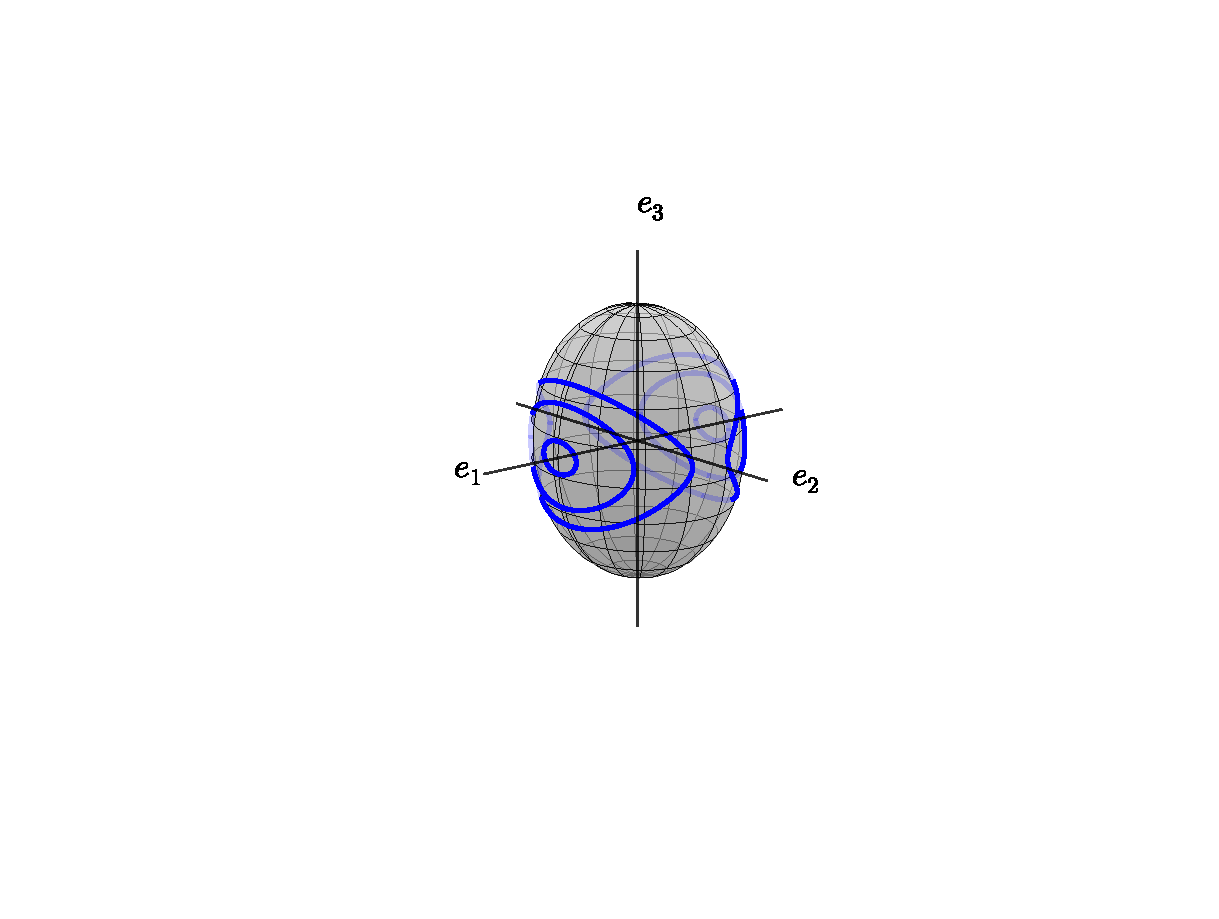
\includegraphics[trim = 70mm 50mm 50mm 20mm, clip=true, width=0.3\textwidth]
             {Ellipsoid_Sphere_low.pdf}} & 
    \subfloat[$ J^{2} = 2EI_{0}$]
             {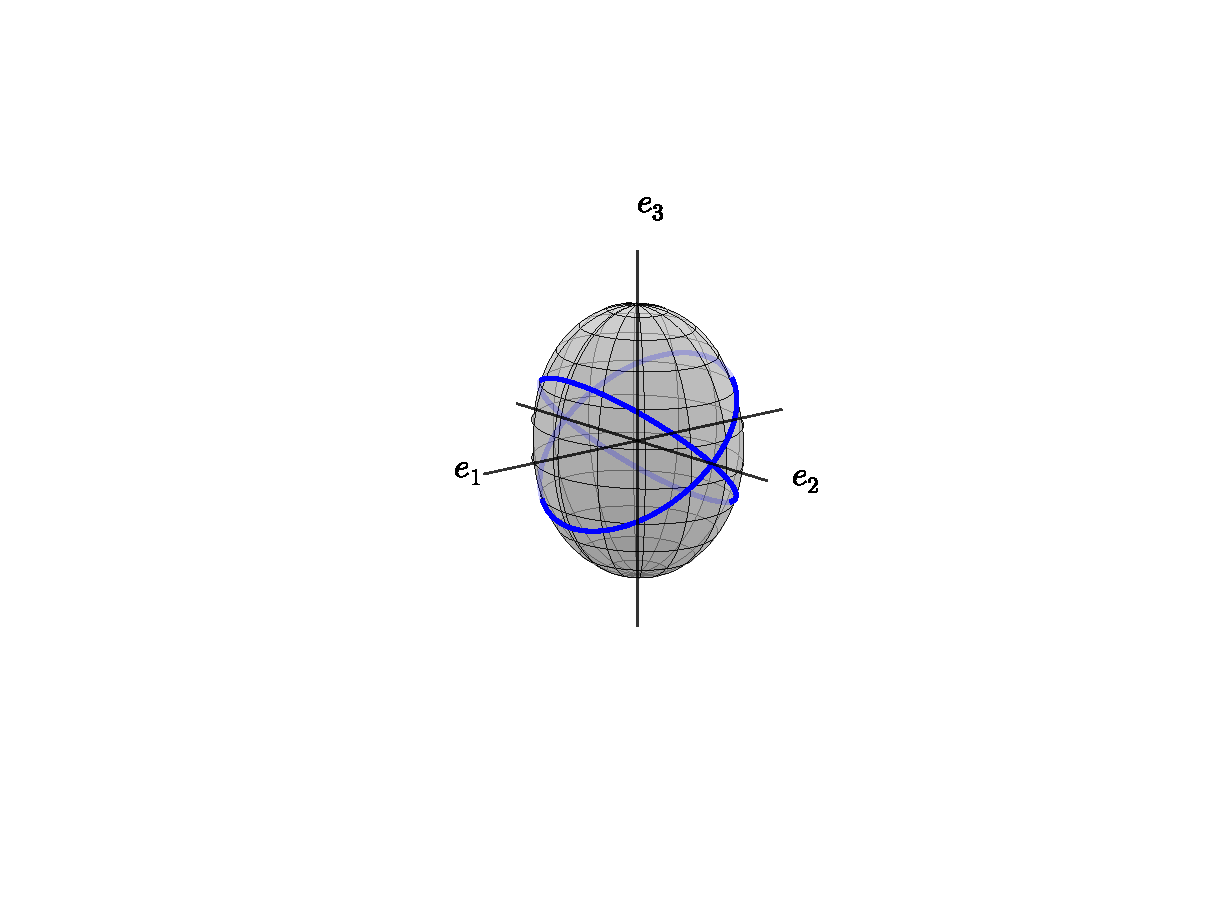
\includegraphics[trim = 70mm 50mm 50mm 20mm, clip=true, width=0.3\textwidth]
             {Ellipsoid_Sphere.pdf}} &
    \subfloat[$2EI_{2}<J^{2}<2EI_{3}$]
             {\includegraphics[trim=70mm 50mm 50mm 20mm, clip=true ,width=0.3\textwidth]
             {{Ellipsoid_Sphere_high}.pdf}}
\end{tabular}
\caption{Intersection of the sphere and ellipsoid defined in equations
    \eqref{eqn: coe} and  \eqref{eqn: com} respectively. }
\label{fig: sphere ellipsoid}
\end{figure}•
We can now relate the three types of intersections to three types of solutions 
for the spin vector.
\begin{enumerate}[(a)]
\item $2E\lambda_{-}<J^{2}<2EI_{0}$ In this region curves form two sets of
    complete loops around the $\1$ axis. As $J^{2} \rightarrow 2E\lambda_{-}$
    the intersection loops will close up about the $\1$ axis.
\item$ J^{2} = 2EI_{0}$ A special case in which the intersection forms two
    closed ellipses
\item  $2EI_{0}>J^{2}>2E\lambda_{+}$ In this region curves form two sets of
    complete loops around the $\3$ axis. As $J^{2} \rightarrow 2E\lambda_{+}$
    the intersection loops will close up about the $\3$ axis.
\end{enumerate}

\FloatBarrier
All simulations begin in the same initial state. As previously observed,
changing $\chi$ through the critical value changes the sign of $\dot{A}$ and
hence whether the sphere will grow or shrink with respect to the ellipsoid. So
for $\chi=30^{\circ}$ the sphere grows with respect to the ellipsoid
($\dot{A}>0$) ending up with the loops closing up about the $\3$ axis. For
$\chi=75^{\circ}$ the sphere shrinks with respect to the ellipsoid
($\dot{A}<0$) ending up with the loops closing up about the $\1$ axis. The two 
end states are then the (a) and (c) pictures in figure \ref{fig: sphere ellipsoid}.

If they both begin from the same initial configuration, then one of them must pass through
the special $J^{2}=2EI_{0}$ state corresponding to figure \ref{fig: sphere ellipsoid}.
When this happens, we will observe a chnage in the axis about which the solution
precesses.

Both sets of solution start with the solution precessing about the $\3$ axis
($\phi$ monotonically increasing) corresponding to figure \ref{fig: sphere ellipsoid}(c) 
In figure~\ref{fig: NS A}(b) the discontinuity is in fact exactly the point
when the solution changes the axes of precession.

To better understand this, we plot the data from the
$\chi=75^{\circ}$ simulation (\ref{fig: NS A}(b)) in figure~\ref{fig: NS A 3D}. Firstly in (a)
we project the spherical components onto the unit sphere and choose three
short sections of data. This shows that at early times, in blue, the solution
precesses about the $\3$ axis. During the discontinuity, in red, the solution
shows similarities with the $J^{2}=2EI_{0}$ case from figure~\ref{fig: sphere
ellipsoid}. Finally at late times, in black, the solution precesses about
the~$\1$~axis. In figure~\ref{fig: NS A 3D}(b) we also plot the solution in
3D during the apparent discontinuity. This again shows the solution goes
through a change of the axis about which it precesses.

\begin{figure}
\centering
\begin{tabular}{cc}
    \subfloat[]{\includegraphics[trim = 30mm 30mm 30mm 30mm, clip=true , width=0.495\textwidth]{{Angle_Space_Plot_3D_chi_75.0_epsI_1.0e-9_epsA_5.0e-11_omega0_1.0e4_eta_1.0e-4}.png}} & 
    \subfloat[]{\includegraphics[trim = 30mm 30mm 30mm 30mm, clip=true , width=0.495\textwidth]{{ThreeD_Plot_Cartesian_chi_75.0_epsI_1.0e-9_epsA_5.0e-11_omega0_1.0e4_eta_1.0e-4}.png}}
\end{tabular}
\caption{Numerical solutions for NS A plotted on the unit sphere in the
body frame axis. (a) shows three distinct time steps: blue, the time before the
discontinuity, red is during the discontinuity and black is some time after.
(b) demonstrates the solution during the discontinuity, the changing colour is
used to illustrate the evolution with time.}
\label{fig: NS A 3D}
\end{figure}•

\FloatBarrier
\subsubsection{NS B in region $\tau_{S}> \tau_{P}>\tau_{A}$}
\label{sec: B}

This NS takes on a new significance having included the anomalous torque:
we can now make a comparison with the work of \citet{Melatos2000}. In this
work, Melatos found that when the precession timescale and anomalous torque
timescales are comparable the solution admits persistent precession. This was
defined as the polar angle $a$ tending to a constant non-zero value with the
nutation amplitude (oscillations in $a$) either decaying or remaining constant.
Because the spin vector has not aligned with a principle axis of the moment of
inertia this was interpreted as the spin vector undergoing persistent
precession. Working in the body frame axis we confirm that $a\ne\pi/2$ at the
end of the evolution in figure~\ref{fig: NS B}(a). 

Transforming to the effective body frame in figure~\ref{fig: NS B}(b) we
find that the spin vector in fact aligns with the principle axis of the
effective moment of inertia ($a \rightarrow \pi /2$.  Therefore the persistent
precession angle found by Melatos is precisely the angle $\beta$. If the
effective moment of inertia tensor is to be believed, then there is no
persistent precession. The spin vector aligns aligns with the principle axis of
the effective moment of inertia tensor associated with the smallest eigenvalue. 

\begin{figure}[ht]
\centering
\begin{tabular}{cc}
    \subfloat[In the body frame axis]
             {\includegraphics[width=0.495\textwidth]
             {{Spherical_Plot_chi_75.0_epsI_4.0e-11_epsA_5.0e-11_omega0_1.0e4_t1_2.0e8}.png}} &
    \subfloat[In the effective body frame axis]
             {\includegraphics[width=0.495\textwidth]
             {{Spherical_Plot_Transform_chi_75.0_epsI_4.0e-11_epsA_5.0e-11_omega0_1.0e4_t1_2.0e8}.png}}
\end{tabular}
\caption{Plot of the spherical components of $\boldsymbol{\omega}$ for NS B}
\label{fig: NS B}
\end{figure}•

\FloatBarrier

\subsubsection{NS C in region $\tau_{P}> \tau_{S}>\tau_{A}$}
\label{sec: C}

For all values of $\chi$ the spin vector is found to align with $1$.  In this
limit ($\epsilon_{A} \gg \epsilon_{I}$ in figure~\ref{fig: beta}) the $\1$ axis
aligns with the magnetic dipole, this agrees with the results for a spherical
star ($\epsilon_{I} \rightarrow 0$). The addition of the anomalous torque
introduces oscillations on the anomalous torque timescale. 

\begin{figure}[ht]
\centering
\begin{tabular}{cc}
    \subfloat[$\chi=30^{\circ}<\chi_{cr}$]{\includegraphics[width=0.495\textwidth]
             {{Spherical_Plot_Transform_chi_30.0_epsI_1.0e-15_epsA_5.0e-11_omega0_1.0e4_t1_1e8}.png}} &
    \subfloat[$\chi=75^{\circ}>\chi_{cr}$]{\includegraphics[width=0.495\textwidth]
             {{Spherical_Plot_Transform_chi_75.0_epsI_1.0e-15_epsA_5.0e-11_omega0_1.0e4_t1_1e8}.png}}
\end{tabular}
\caption{Plot of the spherical components of $\boldsymbol{\omega}$ for NS
C. }
\label{fig: NS C}
\end{figure}•

\FloatBarrier

\subsection{Conclusion: Alignment of the spin vector}
This simple model, comprising an elastic body supporting a biaxial strain and
acted on by an electromagnetic torque, has been validated against known
analytic results. Neglecting the anomalous torque we expand on the results of
\citet{Goldreich1970}: the dependency on $\chi$ of the spin vector alignment is
related to the ratios of angular momentum and energy. 

When using the anomalous torque we introduce the effective body frame. 
In all cases we find that the spin vector aligns with
the principle axis of the effective moment of inertia tensor. For NSs in
region A of figure~\ref{fig: phase space} the effective moment of inertia tensor
is triaxial. This means that it is possible for the spin vector to precess
about either of the principle axis associated with the smallest and largest
eigenvalue. As a result solutions can admit apparent discontinuities, under
inspection these are revealed as the points where the precession changes
between the two axis. 

\section{Connection with the known NS population}
\label{sec: Connection with the known NS population}
TBD
%\label{sec: connection with pp}
%
%Having an understanding of how the different types of solutions behave, we now
%compare this with the known NS population to estimate which types of solutions
%are physically relevant.
%
%Using a large value of the initial spin period will skew the phase diagrams in
%figure \ref{fig: phase space}. We therefore present a more realistic phase
%diagram in figure~\ref{fig: phase space for actual spin frequency} for a
%realistic spin frequency of $\nu=1.6$~Hz. The strongest candidates displaying a
%periodic signal, which may be explained by precession, were collected in
%\citet{Lyne2010}. The 18 NSs where listed along with their: spin frequency,
%frequency derivative and the peak fluctuation frequency of the power spectra
%$F$. It is a standard calculation to find the magnetic field from the first two
%parameters:
%
%\begin{equation}
%B_{s} = 3.3 \times^{19}\sqrt{-\dot{\nu}\nu^{-3}},
%\end{equation}
%see \citet{Lyne2012book} for more details. We now make the assumption that the
%fluctuations at frequency $F$ are due to free precession such that the elastic
%deformation may be calculated by rearranging equation \ref{fig: free
%precession}:
%\begin{equation}
%\epsilon_{I} = \frac{1}{\nu F}.
%\end{equation}•
%We use this as a first approximation to discuss the types of solution that may
%be relevant to the NS population, but recognise that we have yet to account
%for the damping due to any superfluid core.
%\begin{figure}[ht]
%\centering
%	\centering
%    \includegraphics[width=0.6\textwidth,trim=0mm -10mm 0mm 0mm]
%                    {{Phase_Space_Realistic_Omega0}.png}
%\caption{Phase space of the orderings of the three timescales using a realistic
%    value of the spin frequency. This can be compared with estimates of where
%    the NSs from \citet{Lyne2010} sit assuming the periodic oscillations
%are due to precession.}
%\label{fig: phase space for actual spin frequency}
%\end{figure}•
%Plotting the results in figure~\ref{fig: phase space for actual spin frequency} we observe that all NSs exist in Region A of the phase diagram. 
%
%\FloatBarrier
%
%\subsection{Future work}
%Having validated that our simple framework  agrees with the results in the
%literature we can look forward to see how it may be used and what is not yet
%included. Recent work by \citet{Seymour2012} has found evidence for chaotic
%behaviour in several NSs, they predict that the governing equations should
%be 3 non linear coupled ODEs with one variable the spin down. Our model fits
%such a system and so we aim to search for any chaotic behaviour in our results
%and use this as an observational test of out model. The primary objection to
%precession as an underlying mechanism for timing noise is that any fluid core
%of the NS will damp the precession. We aim to reproduce this result by
%adding a second core following the frictional coupling method of
%\citet{Bondi1955}. Adding random kicks during the spin down we can  evaluate
%the suggestion of \citet{Cordes1993} that such kicks will excite the
%precession. In addition we can check the ideas of \citet{Cordes2013} that the
%periodicity results from stochastic resonance. Comparing the size and frequency
%of kicks with realistic models  will help to ascertain the validity of this
%idea. 

\appendix
\begin{subappendices}
\section{Goldreich's result}
\label{sec: goldreich}
Starting with 
\begin{equation}
A=\frac{M^{2}}{2EI_{0}},
\end{equation}
and differentiating
\begin{equation}
\dot{A}=\frac{1}{(2EI_{0})^{2}}
        \left(\frac{d}{dt}(M^{2})2EI_{0}-\frac{d}{dt}(2EI_{0})M^{2}\right),
\end{equation}
simplifying and writing in index notation we have
\begin{equation}
\dot{A}=\frac{1}{E^{2}}\left(2M^{i}\dot{M}_{i}E-\dot{E}M^{i}J_{i}\right).
\end{equation}
Now $E=\frac{1}{2}I_{ij}\omega^{i}\omega^{j}$,  $\dot{E}=T^{i}\omega_{i}$ and
$\dot{M}^{i}=T^{i}$, and so
\begin{equation}
\dot{A}=\frac{1}{E^{2}}\left(M^{i}T_{i}I_{jk}\omega^{j}\omega^{k}
                             -T^{i}\omega_{i}M^{j}J_{j}\right).
\end{equation}
For a diagonalised matrix, $I_{ij}$ has only 3 non zero components and so
$I_{jk}\omega^{j}\omega^{k}=(I\omega)_{j}\omega^{j}$. In addition
$M^{i}=(I\omega)^{i}$ and so writing
\begin{equation}
\dot{A}=\frac{1}{E^{2}}T^{i}\left((I\omega)_{i}\omega_{j}
        -\omega_{i}(I\omega)_{j}\right)(I\omega)^{j},
\end{equation}
\begin{equation}
\dot{A}=\frac{1}{E^{2}}T^{i}\omega_{i}\omega_{j}
        (I\omega)^{j}\left(I^{i}_{\;i}-I^{j}_{\;j}\right).
\end{equation}
Considering for the time being only the last few terms and expanding the
summation it is clear all $i=j$ terms will be zero. Working with a biaxial mass
distribution where $I_{1}=I_{2}$, then the only non-zero terms are given by 
\begin{eqnarray*}
T^{i}\omega_{i}\omega_{j}(I\omega)^{j}\left(I^{i}_{\;i}-I^{j}_{\;j}\right)&=&
T_{1}\omega_{1}I_{0}(1-\epsilon_{i})\omega^{2}_{3}
(I_{0}-I_{0}(1+\epsilon_{I}))+
T_{2}\omega_{2}I_{0}(1-\epsilon_{i})\omega^{2}_{3}(I_{0}-I_{0}(1+\epsilon_{I})) 
\\ && + 
T_{3}\omega_{3}(I_{0}(1+\epsilon_{I})-I_{0})
               (I_{0}\omega_{1}^{2}+I_{0}\omega_{2}^{2}), \\
&=& I_{0}^{2}\epsilon_{I}\omega_{3}\left(T_{3}(\omega_{1}^{2}+\omega_{2}^{2}) 
    - \omega_{3}(1+\epsilon_{I})(T_{1}\omega_{1}+T_{2}\omega_{2})\right).
\end{eqnarray*}
Working up to 1st order in $\epsilon_{I}$ and inserting the spherical polar
coordinates and then the spindown torque (we neglect the anomalous torque here)
we have
\begin{eqnarray*}
&=& I_{0}^{2}\epsilon_{I}\omega^{3}
    \left(\frac{2R}{3c}\epsilon{A}\omega^{3}\right)
    \cos a \left([\sin \chi \cos \chi \sin a \cos \phi 
                 - \sin^{2}\chi \cos a]\sin^{2} a \right. \\
&& \left.- \cos a ([\sin \chi \cos \chi \sin a \cos \phi 
                   - \sin^{2}\chi \cos a]\cos \phi \sin a 
                   - \sin^{2}a \sin^{2}\phi)\right).
\end{eqnarray*}
Of course to know the exact behaviour, one would need to fully solve the
original ODEs. To show agreement with Goldreich's result, we can assume that
$\phi$ varies much faster than $a$ and $\omega$ such that $\tau_{P}<<\tau_{S}$.
Then averaging over a free nutation period and neglecting the coefficients for
the time being
\begin{eqnarray*}
&\sim& \cos a \left(-\sin^{2}a\cos a \sin^{2}\chi + 
       \frac{1}{2}\left(\sin^{2}a\cos a \cos^{2}\chi + 
       \sin^{2}a \cos a \right) \right) \\
& \sim& \cos^{2} a \sin^{2}a\left(1-\frac{3}{2}\sin^{2}\chi\right).
\end{eqnarray*}
Finally putting all the terms together we have an expression for the averaged
rate of change of $A$ with respecting Goldreich's assumptions:
\begin{equation}
\langle \dot{A} \rangle =\frac{1}{\langle E\rangle ^{2}}I_{0}^{2}
                         \epsilon_{I}\omega^{6}\frac{2R}{3c}\epsilon{A} 
                         \cos^{2} a \sin^{2}a
                         \left(1-\frac{3}{2}\sin^{2}\chi\right) 
\end{equation}

\section{Considerations for the timescales}\label{sec: timescales}
We have used the ordering of the three timescale at $\omega_{0}=\omega(t=0)$
to categorise the results. However, clearly the magnitude of the spin vector
will decrease and the different dependencies on the spin vector could cause a
`crossing' of the timescales producing unexpected results. Writing the
timescales then as 
\begin{equation}
\tau_{P}(t)=\frac{2\pi}{\epsilon_{I}\omega(t)}, \;\;\;\;\; 
\tau_{A}(t)=\frac{2\pi}{\epsilon_{A}\omega(t)},  \;\;\;\;\; 
\tau_{S}(t)=\frac{3c}{2R}\frac{2\pi}{\epsilon_{A}\omega(t)^{2}}.
\end{equation}
Only $\tau_{S}$ could cross with the other two timescales since the spin down
and anomalous timescales obey $\tau_{S}>\tau_{A}$ provided that 
\begin{equation*}
\omega(t)>\frac{3c}{2R}.
\end{equation*}•
This condition is satisfied by setting the initial rotational spin frequency at
less than $\omega_{0} \sim 10^{4}$ [Hz rad], that is the star should not break
special relativity. At later times the spin frequency will decay and so this
condition is still satisfied.

For the anomalous torque and precession timescale crossings two cases exists:
either the deformations are such that the spin down timescale is larger than
the precession initially (region A and B) or, as in region C, the precession
timescale is larger than then spin down timescale. Considering the first case:
\begin{equation}
\tau_{S}>\tau_{P} \;\;\; 
\Rightarrow \omega(t)<\frac{3c}{2R}\frac{\epsilon_{I}}{\epsilon_{A}}.
\end{equation}•
In this particular state $\epsilon_{I}>\epsilon_{A}$ and so as in the previous
case while the spin vector decays this inequality is always satisfied and the
orderings remain the same. In the other case we have:
\begin{equation}
\tau_{P}>\tau_{S} \;\;\; 
\Rightarrow \omega(t)>\frac{3c}{2R}\frac{\epsilon_{I}}{\epsilon_{A}}.
\end{equation}
In this case it is possible for the time scales to cross at
$\omega_{cr}=\frac{3c}{2R}\frac{\epsilon_{I}}{\epsilon_{A}}$. For pulsar C this
corresponds to a rotational spin frequency of $0.9$ [Hz rad] which is four
orders of magnitude smaller than the initial freuquency. For this reason we can
rule out this crossing of the time scales as an important factor in
calculations. 



\end{subappendices}
\biblio

\end{document}
